\documentclass{article}
\usepackage{tikz}
\usetikzlibrary{arrows.meta}

\begin{document}

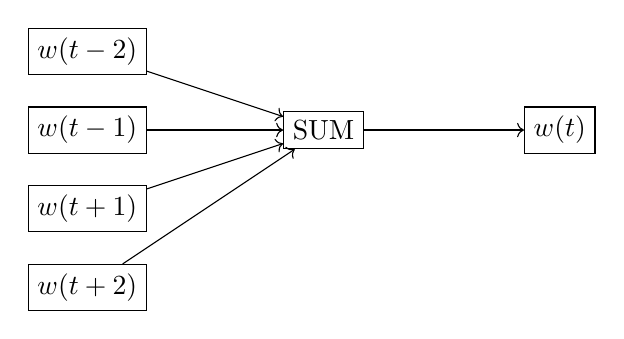
\begin{tikzpicture}[node distance=1cm]
    % Define nodes
    \node (w_t_minus_2) [draw] {$w(t-2)$};
    \node (w_t_minus_1) [draw, below of=w_t_minus_2] {$w(t-1)$};
    \node (w_t_plus_1) [draw, below of=w_t_minus_1] {$w(t+1)$};
    \node (w_t_plus_2) [draw, below of=w_t_plus_1] {$w(t+2)$};
    \node (sum) [draw, right of=w_t_minus_1, node distance=3cm] {SUM};
    \node (w_t) [draw, right of=sum, node distance=3cm] {$w(t)$};

    % Draw arrows
    \draw[->] (w_t_minus_2) -- (sum);
    \draw[->] (w_t_minus_1) -- (sum);
    \draw[->] (w_t_plus_1) -- (sum);
    \draw[->] (w_t_plus_2) -- (sum);
    \draw[->] (sum) -- (w_t);
\end{tikzpicture}

\end{document}